\documentclass[border=3pt]{standalone}
% Preâmbulo compartilhado pelos diagramas TikZ da aula 8 de IHR (Métodos de Pesquisa)
\usepackage[T1]{fontenc}
\usepackage[utf8]{inputenc}
\usepackage{lmodern}
\usepackage{amsmath}
\usepackage{xcolor}
\usepackage{tikz}
\usetikzlibrary{arrows.meta,angles,quotes,decorations.pathmorphing,decorations.pathreplacing,calc,
                positioning,shapes.geometric,shapes.misc,backgrounds,fit,
                math}

% Paleta (mesma dos SVGs originais)
% Paleta da disciplina de IHR: acento azul (#1A6FB5), cor de destaque do tema.
% (o nome "dblue" é mantido para não alterar todos os diagramas)
\definecolor{dblue}{HTML}{1A6FB5}
\definecolor{dorange}{HTML}{B3541E}
\definecolor{dgreen}{HTML}{4A7C59}
\definecolor{dred}{HTML}{9C4B4B}
\definecolor{dcream}{HTML}{F4F1EA}
\definecolor{dshade}{HTML}{DDD7C9}

% Função gaussiana (não normalizada por padrão de escala visual)
\pgfmathdeclarefunction{gauss}{3}{%
  \pgfmathparse{1/(#3*sqrt(2*pi))*exp(-((#1-#2)^2)/(2*#3^2))}%
}

% Estilos comuns (prefixo d... para não colidir com chaves internas do pgf)
\tikzset{
  >={Stealth[length=2mm]},
  dguide/.style={gray!55, dashed, line width=0.4pt},
  daxis/.style={gray!60, line width=0.7pt, ->},
  dbody/.style={fill=black!3, draw=black!80, line width=1pt},
  dacc/.style={draw=dblue, line width=1pt},
  dlbl/.style={black!55, font=\small},
  dsub/.style={black!45, font=\footnotesize},
  dstate/.style={circle, draw=black!80, fill=dcream, line width=1pt,
                 minimum size=17mm, font=\large, inner sep=1pt},
  dobs/.style={circle, draw=black!80, fill=dshade, line width=1pt,
               minimum size=14mm, font=\large, inner sep=1pt},
  dbox/.style={rounded corners=2pt, draw=black!80, fill=dcream, line width=1pt,
               align=center, inner sep=6pt},
  dop/.style={circle, draw=black!80, fill=white, line width=1pt,
              minimum size=6mm, inner sep=0pt, font=\small},
  dtrans/.style={->, dblue, line width=1pt},
  dmeas/.style={->, dorange, line width=1pt},
  dcurve/.style={line width=1pt, dblue},
  dcurveb/.style={line width=1.4pt, dorange},
}

\begin{document}
\hyphenpenalty=10000 \exhyphenpenalty=10000 \tolerance=9999 \emergencystretch=3em
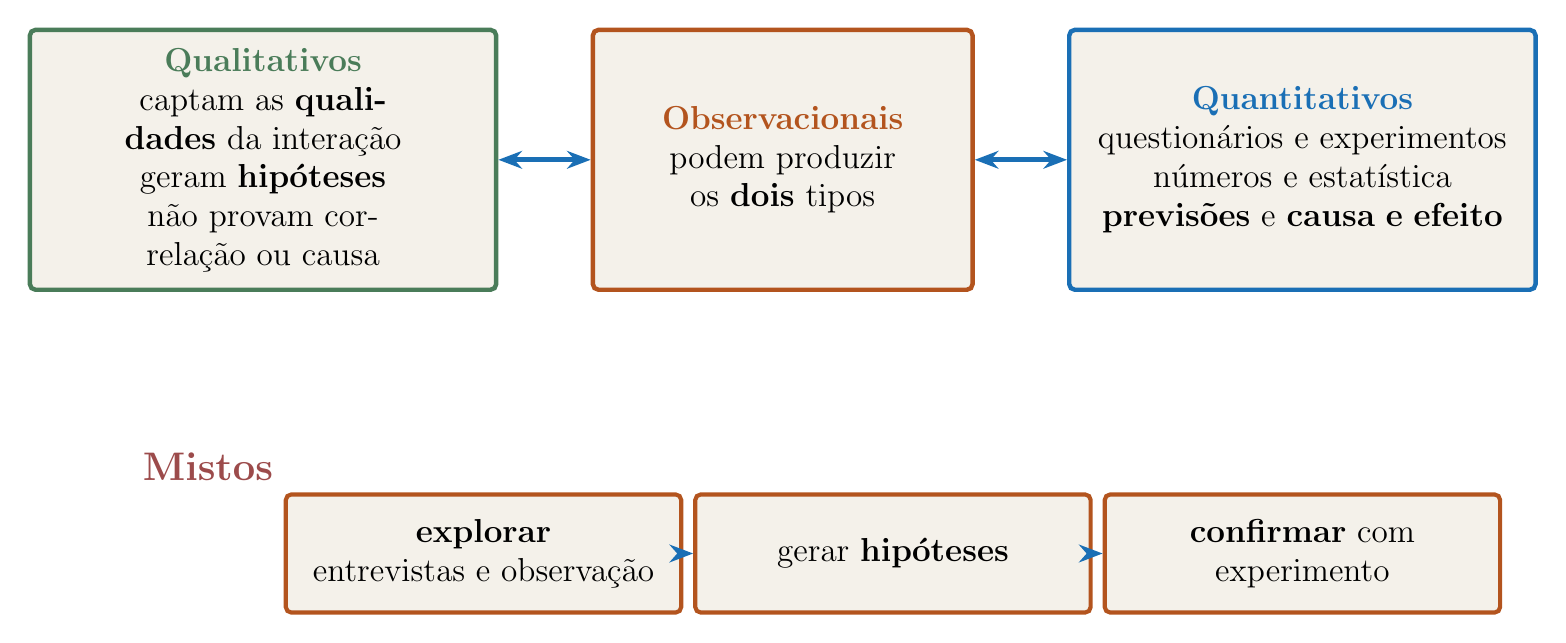
\begin{tikzpicture}[x=1cm,y=1cm]
  \tikzset{c/.style={dbox, text width=5.5cm, minimum height=3.3cm, font=\large, line width=1.6pt, align=center}, e/.style={dbox, draw=dorange, line width=1.5pt, text width=4.6cm, minimum height=1.5cm, font=\large, align=center}}
  \node[c, draw=dgreen] (q) at (2.9,6.6) {\textbf{\textcolor{dgreen}{Qualitativos}}\\ captam as \textbf{qualidades} da interação\\ geram \textbf{hipóteses}\\ não provam correlação ou causa};
  \node[c, draw=dblue] (n) at (16.1,6.6) {\textbf{\textcolor{dblue}{Quantitativos}}\\ questionários e experimentos\\ números e estatística\\ \textbf{previsões} e \textbf{causa e efeito}};
  \node[c, draw=dorange, text width=4.4cm] (o) at (9.5,6.6) {\textbf{\textcolor{dorange}{Observacionais}}\\ podem produzir os \textbf{dois} tipos};
  \draw[dtrans, line width=1.8pt, {Stealth[length=3mm]}-{Stealth[length=3mm]}] (q.east) -- (o.west);
  \draw[dtrans, line width=1.8pt, {Stealth[length=3mm]}-{Stealth[length=3mm]}] (o.east) -- (n.west);
  \node[font=\Large\bfseries, dred] at (2.2,2.7) {Mistos};
  \node[e] (a) at (5.7,1.6) {\textbf{explorar}\\ entrevistas e observação};
  \node[e] (b) at (10.9,1.6) {gerar \textbf{hipóteses}};
  \node[e] (d) at (16.1,1.6) {\textbf{confirmar} com experimento};
  \draw[dtrans, line width=1.8pt, -{Stealth[length=3mm]}] (a.east) -- (b.west);
  \draw[dtrans, line width=1.8pt, -{Stealth[length=3mm]}] (b.east) -- (d.west);
\end{tikzpicture}
\end{document}
